\section{Presentation of the Web-based Platform}

%     interface
%     hosting final product in docker containers and charge balancing with nginx


\subsection{Introduction}
    In this section we are going to talk about the different tools and resources that helped us build our project, we will talk about the software, hardware and explain in detail the features of the web application and finally present the interface.


\subsection{Hardware}
    This project is a 2-person teamwork, we were able to implement it using 2 laptops: \\
    \bigskip \\
    \textbf{Asus vivobook}: with an intel CPU i7 7nth generation with a clock rate of 2.7GHz and an Nvidia GPU GeForce 930mx, 12 GB of RAM and 240 GB of Solid State Drive, with a Linux Mint 20.3 Cinnamon operating system\\ 
    \bigskip \\
    \textbf{Dell XPS}: with a 7th Generation Intel Core i7-7700HQ Quad Core Processor (6M cache, up to 3.8 GHz) and NVIDIA GeForce GTX 1050 4GB DDR5 Graphics that was used to train the CNN model , 16 GB RAM DDR4-2400MHz and 512 GB PCIe Solid State Drive, with a Windows 10 Professional edition operating system \\ 


\subsection{Software}
    The implementation of the project was achieved using various frameworks and libraries, and from those we mention the following: \\
    \footnotesize
    \begin{itemize}
        \item \textbf{JSON} : Stands for JavaScript Object Notation. is a lightweight format for storing and transporting data. It is easy for humans to read and write. ~\cite{4}
        \item \textbf{YAML} : Is a data serialization language that is often used for writing configuration files. It is human-readable and easy to understand. ~\cite{5}
        \item \textbf{HTTP} : Stands for Hyper Text Transfer Protocol. is the foundation of the World Wide Web, and is used to load web pages using hypertext links. ~\cite{6}
        \item \textbf{RESTful API}: Is an interface that two computer systems use to exchange information securely over the internet. ~\cite{7}
        \item \textbf{Web Server}: A web server stores and delivers the content for a website content to clients that request it. is substantially used to host the web sites. ~\cite{8}
        \item \textbf{Reverse} Proxy : Is a server that sits in front of web servers and forwards client requests to those web servers. It is typically  used to help increase security, performance, and reliability. ~\cite{9}
        \item \textbf{SSH} : Stands for Secure Shell. is a network protocol that helps us securely access and communicate with remote machines (mostly remote servers). ~\cite{11}
        \item \textbf{AWS} : Stands for Amazon Web Services. It is a platform that offers flexible, reliable, scalable, easy-to-use and cost-effective cloud computing solutions. ~\cite{12}
        \item \textbf{Python} : Python is an interpreted, object-oriented, high-level programming language with dynamic semantics. It is preferred for programming due to its vast features, applicability, and simplicity. The Python programming language best fits machine learning due to its independent platform and its popularity in the programming community. ~\cite{15}
        \item \textbf{Numpy} : "Stands for Numerical Python. Numpy is a Python library consisting of multidimensional array objects and a collection of routines for processing those arrays. Using NumPy, mathematical and logical operations on arrays can be performed." ~\cite{16}
        \item \textbf{Pandas} : It is a Python library that is most widely used for machine learning and data science tasks. It is provided on the top of  Numpy, which provides support for multi-dimensional arrays. ~\cite{17}
        \item \textbf{Matplotlib} : It is a data visualization and graphical plotting library for Python. It makes easy things easy and hard things possible. ~\cite{18}
        \item \textbf{Pillow} : It is a fork of PIL, Stands for Python Imaging Library. It is the standard image processing package for the Python programming language. It includes lightweight image processing capabilities that help with image creation, editing, and saving. ~\cite{19}  
        \item \textbf{Tensorflow}: It is an open-source platform developed by Google Brain Team. It is entirely based on the Python programming language and used for numerical computation and data flow, which makes creating and deploying machines and deep learning models faster and easier. ~\cite{20}
        \item \textbf{Keras}: It is a deep learning API written in Python, running on top of the machine learning platform TensorFlow, Keras simplifies the implementation of complex neural networks with its easy to use framework. ~\cite{21}
        \item \textbf{CUDA}: It is a parallel computing platform and an API model that was developed by NVIDIA. CUDA enables developers to speed up compute-intensive applications by harnessing the power of GPUs for the parallelizable part of the computation. ~\cite{22}  
        \item \textbf{cuDNN}: Stands for CUDA Deep Neural Network. It is a low-level library that provides GPU kernels frequently used in deep learning. cuDNN  provides highly tuned implementations for standard routines such as forward and backward convolution, pooling, normalization, and activation layers. ~\cite{23}
        \item \textbf{Anaconda}: It is a distribution of the Python and R programming languages that is open-source and free. The Python interpreter and a number of machine learning and data science-related packages are included in the distribution. For those interested in those fields, Anaconda makes it simple to install all (or the majority) of the required packages with a single installation. ~\cite{24}
        \item \textbf{Jupyter Notebook}: "It is a free, open-source, interactive web tool known as a computational notebook, which researchers can use to combine software code, computational output, explanatory text and multimedia resources in a single document." ~\cite{25}
        \item \textbf{JavaScript}: It is a dynamic computer programming language used both on the client-side and server-side that allows you to create more dynamic interactions when developing web pages, applications, servers, and or even games. ~\cite{26}  
        \item \textbf{React}.js: It is a JavaScript library that is open-source and used to create user interfaces specifically for single-page applications. It is utilized to manage the view layer for web and mobile applications. We can design reusable UI components with React as well. ~\cite{27}
        \item \textbf{Material}-UI: It is a library that allows us to import and use different components to create a user interface in our React applications. ~\cite{277}
        \item \textbf{Mongoose}: It is an Object Data Modeling (ODM) library for MongoDB and Node.js. It manages relationships between data, provides schema validation, and is used to translate between objects in code and the representation of those objects in MongoDB.
        \item \textbf{Dart}: Dart is an open-source, general-purpose, object-oriented programming language developed by Google. It is used with Flutter to build mobile, web and  apps. This is one of the most common uses of Dart today. ~\cite{28}        
        \item \textbf{Flutter}: Flutter is a free and open-source mobile UI framework created by Google. it allows you to create a native mobile, desktop, and web apps with a single codebase. This means that you can use one programming language and one codebase to create different apps. ~\cite{29}
        \item \textbf{Node}.js: It is an open-source, cross-platform runtime environment built on Chrome's V8 JavaScript engine that allows developers to create all kinds of server-side tools and applications in JavaScript. ~\cite{30}
        \item \textbf{MongoDB}: It is a non-relational document database that supports storage which is similar to JSON. The MongoDB database offers full indexing support, replication, and a flexible data model that makes it possible to store unstructured data. It also has rich and user-friendly APIs. ~\cite{31}
        \item \textbf{Express}.js: It  is a free and open-source web application framework for Node.js. It is used for designing and building web applications quickly and easily. ~\cite{32}
        \item \textbf{Flask}: It is a microframework that provides libraries to build lightweight web applications in python. ~\cite{33}
        \item \textbf{Slack}: "It is essentially a chat room designed to replace email as your primary method of communication and sharing. Its workspaces allow you to organize communications by channels for group discussions and allows for private messages to share information, files, and more all in one place." ~\cite{34}
        \item \textbf{Github}: "It is an online software development platform used for storing, tracking, and collaborating on software projects. It enables developers to upload their own code files and to collaborate with fellow developers on open-source projects." ~\cite{35}
        \item \textbf{Nginx}: "It is open source software for web serving, reverse proxying, caching, load balancing, media streaming, and more. It started out as a web server designed for maximum performance and stability." ~\cite{36}
        \item \textbf{Docker}: "is an open platform for developing, shipping, and running applications. Docker enables you to separate your applications from your infrastructure so you can deliver software quickly. With Docker, you can manage your infrastructure in the same ways you manage your applications. By taking advantage of Docker’s methodologies for shipping, testing, and deploying code quickly, you can significantly reduce the delay between writing code and running it in production." ~\cite{37}
        \item \textbf{EC2}: "Stands for Elastic Compute Cloud. It provides scalable computing capacity in the Amazon Web Services (AWS) Cloud. Using Amazon EC2 eliminates your need to invest in hardware up front, so you can develop and deploy applications faster." ~\cite{38}
    \end{itemize}
    \normalsize
\subsection{The Web Application}
    \subsubsection{Authentication}
        The Authentication was implemented using JWTs (JSON web tokens) which is acquired by the frontend client after Logging in or Signing up, after that it will be saved in a session storage and sent as an Authorization header with each request that requires authentication, in the backend the tokens are saved in an array to allow for multiple session communication, which means that a user can connect from multiple devices, with the ability to logout from all sessions being available in the profile settings.
    
    \subsubsection{Permissions and Roles}
        There are mainly 3 roles in our application: Admin, Doctor, User. Each one of these roles comes with a certain level of access. The permissions were implemented using ExpressJS middleware, the list of permissions goes as follows, 

        \begin{description}
            \item[Admin]:\\
            \begin{itemize}
                \item User management.
                \item View all doctors
                \item Doctor verification, through credentials sent by e-mail.
            \end{itemize}
            \item[Doctor]:\\
            \begin{itemize}
                \item View published lesions.
                \item Comment on a published lesion
                \item Communicate with a patient
            \end{itemize}
            \item[User]:\\
            \begin{itemize}
                \item Profile management.
                \item Upload a lesion.
                \item Publish/Unpublish a lesion
                \item View own lesions
                \item Comment  on own lesion
                \item Communicate with a doctor 
            \end{itemize}
        \end{description}
    
        Keep in mind that the Admin also has the permissions of the doctor, and a Doctor also has the permissions of a normal user.

    \subsubsection{Communications Between Different Parts Of The Application}
        We divided our application 2 frontends and 2 backends and a database, 2 frontend clients one for a browser(ReactJS) and one for a smartphone (Flutter), these 2 communicate with the main backend (NodeJS) using Rest API architecture and http/https protocol. and the main backend communicates with the 2nd backend (flask) which has the implementation of the CNN prediction model also using Rest API architecture and http/https protocol, and with the database server using MongoDB protocol.

        The CNN model is used when a user uploads a lesion image to the NodeJS backend, and after that the Node server sends the image to the model and receives a prediction string from it which after that saved in the database and returned to the frontend client.

    \subsubsection{Hosting}
    As it is show in the deployment diagram figure ~\ref{fig:dep}, we have hosted our project in an AWS EC2 server combined with Docker, in other words, the Docker engine is hosted in AWS and our software parts are distributed  in various docker containers.
    We have chooses docker to facilitate the deployment process, and benefit from the DNS server provided inside the docker engine between the containers, which allows us to use host names to connect different parts of our software instead of IP addresses, docker also provides better resource consumption and better network security that allows us to control what we expose to the public. Containers are easy to maintain, a change in one container will not affect the other containers, and as a final point if we ever decide to change the hosting provider docker makes that easy, all we need is the configuration of docker and the data of our users, and we are all set.

    \subsection{The Interface}
        We present the application's interface in the following figures: 
        % ---login 
        % ---signup
        % profile
        %     lesions
        %         ---upload 
        %         ---previous lesions
        %     settings
        %         ---upload photo
        %         delete photo
        %         ---delete account
        %         logout all
        % ---forum
        % ---messages
        % dashboard
        %     ---doctors, verify unverify
        %     users, delete



        % \begin{figure}[H]
        % \begin{center}
        % \includegraphics[width=12cm]{./diagnosis-system/presentation-of-app/.png}
        % \end{center}
        % \caption{}
        % \label{fig:}
        % \end{figure}

        
        \noindent \textbf{First of all, the following 2 figures demonstrate the Login and Signup interfaces:} \\
        you can log in with Email and Password, or Signup providing Name, Role, Email, Password
        \begin{figure}[H]
        \begin{center}
        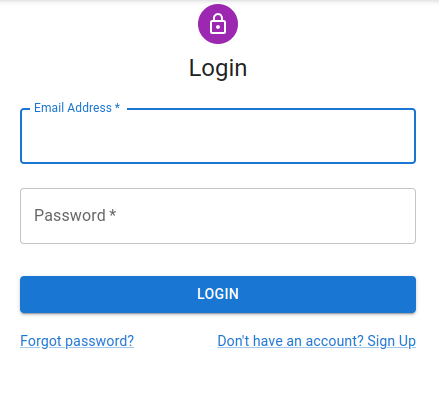
\includegraphics[width=7cm]{./diagnosis-system/presentation-of-app/login.png}
        \end{center}
        \caption{Login}
        \label{fig:}
        \end{figure}

        

        \begin{figure}[H]
        \begin{center}
        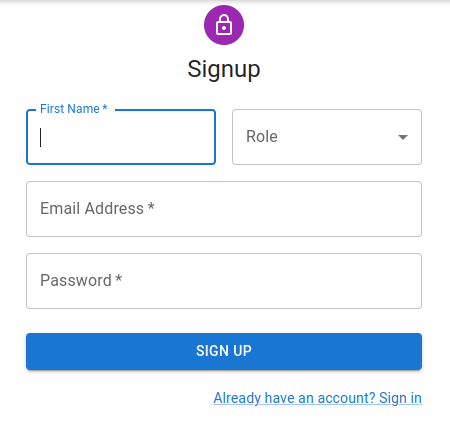
\includegraphics[width=12cm]{./diagnosis-system/presentation-of-app/signup.png}
        \end{center}
        \caption{Signup}
        \label{fig:}
        \end{figure}

        
        \noindent \textbf{The following interfaces are in the Profile page:} \\
        \noindent You can view profile information, upload a profile image, and delete your account 
        \begin{figure}[H]
        \begin{center}
        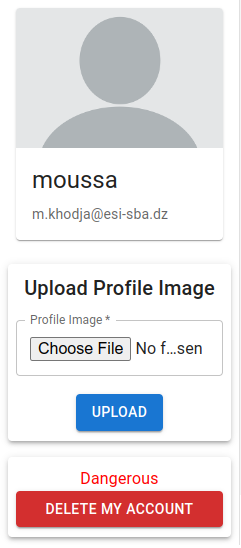
\includegraphics[width=7cm]{./diagnosis-system/presentation-of-app/profile-settings.png}
        \end{center}
        \caption{Profile Settings}
        \label{fig:}
        \end{figure}

        
        \noindent This component allows you to upload a lesion image with a description 
        \begin{figure}[H]
        \begin{center}
        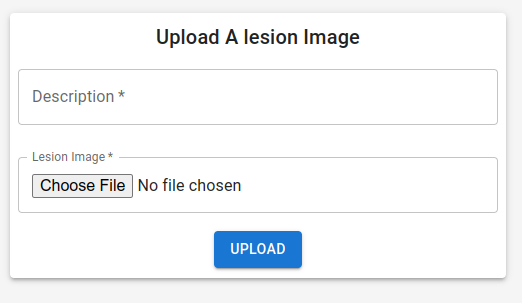
\includegraphics[width=10cm]{./diagnosis-system/presentation-of-app/upload-lesion.png}
        \end{center}
        \caption{Upload a lesion Image, with a description}
        \label{fig:}
        \end{figure}

        
        \noindent \textbf{The following interfaces are found in the Forum page:} \\
        \noindent You can view all lesions that were published by patients, and give your professional opinion by leaving a comment, you can also view comments from other doctors
        \begin{figure}[H]
        \begin{center}
        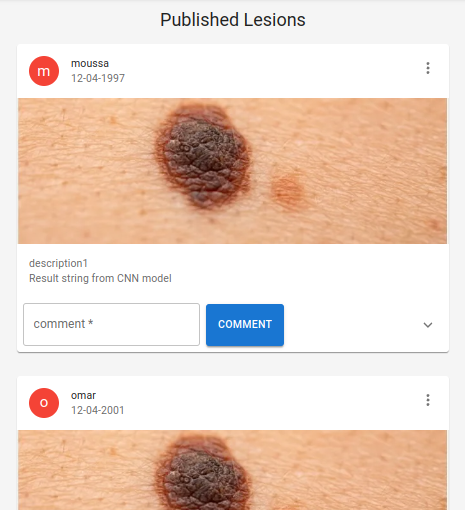
\includegraphics[width=10cm]{./diagnosis-system/presentation-of-app/published-lesions.png}
        \end{center}
        \caption{View published lesions as a doctor}
        \label{fig:}
        \end{figure}

        

        \begin{figure}[H]
        \begin{center}
        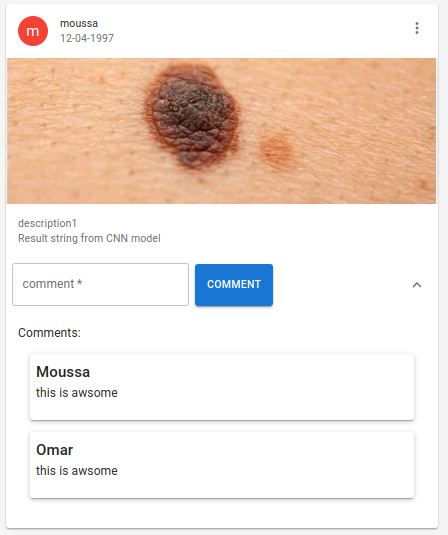
\includegraphics[width=10cm]{./diagnosis-system/presentation-of-app/comment.png}
        \end{center}
        \caption{Comment on a lesion}
        \label{fig:}
        \end{figure}

        
        \noindent \textbf{This interface represents the Communication page:} \\
        You can send and receive messages, between doctors and patients
        \begin{figure}[H]
        \begin{center}
        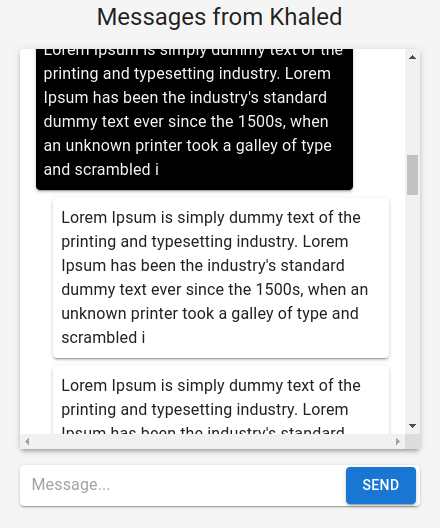
\includegraphics[width=10cm]{./diagnosis-system/presentation-of-app/messeges.png}
        \end{center}
        \caption{Messaging}
        \label{fig:}
        \end{figure}

        
        \noindent \textbf{The following interfaces are found in the dashboard:} \\
        After checking the credentials sent by email, the admin can verify a doctor's account, because a non-verified doctor is considered as a normal user, and he can't access patients information 
        \begin{figure}[H]
        \begin{center}
        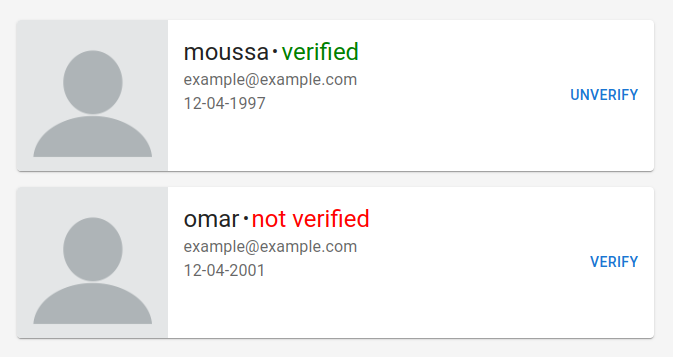
\includegraphics[width=10cm]{./diagnosis-system/presentation-of-app/verify-doctors.png}
        \end{center}
        \caption{View all doctors by Admin + verify/unverify a doctor}
        \label{fig:}
        \end{figure}


        
        
\subsection{Future Work}
    we present these ideas as a future work to extend the usability of our project
    \begin{itemize}
        \item Detect and classify more lesions and not just melanoma.
        \item Take model interpretability into account, so it will be more acceptable in real world scenarios.
        \item Present more in-app features to facilitate and enhance user experience. 
    \end{itemize}